\documentclass[11pt,a4paper]{article}

\usepackage[utf8]{inputenc}
\usepackage[T1]{fontenc}
\usepackage{amsmath,amssymb}
\usepackage{graphicx}
\usepackage{hyperref}
\usepackage{booktabs}
\usepackage{listings}
\usepackage{xcolor}
\usepackage{tikz}
\usetikzlibrary{shapes.geometric, arrows.meta, positioning, fit, backgrounds}
\usepackage[margin=1in]{geometry}
\usepackage{natbib}
\usepackage{algorithm}
\usepackage{algpseudocode}

\definecolor{codegreen}{rgb}{0,0.6,0}
\definecolor{codegray}{rgb}{0.5,0.5,0.5}
\definecolor{codepurple}{rgb}{0.58,0,0.82}
\definecolor{backcolour}{rgb}{0.95,0.95,0.92}

\lstdefinestyle{mystyle}{
    backgroundcolor=\color{backcolour},
    commentstyle=\color{codegreen},
    keywordstyle=\color{codepurple},
    numberstyle=\tiny\color{codegray},
    basicstyle=\ttfamily\footnotesize,
    breaklines=true,
    frame=single,
}
\lstset{style=mystyle}

\title{Software Intent Runtime: A Compiler Architecture for\\LLM-Driven Software Synthesis}

\author{
  Anonymous Author(s)
}

\date{}

\begin{document}

\maketitle

\begin{abstract}
We present \textbf{Software Intent Runtime (SIR)}, a compiler-inspired architecture that frames Large Language Models (LLMs) as compilers translating human intent (a high-level language) into software artifacts (a low-level target). SIR introduces a graph-based Intermediate Representation (IR) that captures software architecture as typed nodes and edges, enabling a multi-stage compilation pipeline: intent parsing, patch generation, graph transformation, adapter lowering, and code generation. Unlike direct code-generation approaches, SIR maintains a persistent, versionable, and validatable architectural state that supports incremental modification, structural validation, and deterministic code emission. We describe the system design, formalize the IR semantics, and demonstrate the pipeline through a working implementation. Our results show that the compiler metaphor provides a principled foundation for LLM-driven software engineering that improves traceability, correctness, and composability over single-shot generation.
\end{abstract}

\section{Introduction}

The rapid advancement of Large Language Models (LLMs) has created a paradigm shift in software engineering. Tools such as GitHub Copilot, Cursor, and Claude Code can generate, modify, and debug code from natural language descriptions. However, current approaches overwhelmingly treat code generation as a \emph{translation} problem---mapping natural language directly to source code in a single pass.

We argue that this framing misses a fundamental insight: \textbf{LLMs are compilers}. In the classical compiler pipeline, a high-level language is parsed into an abstract syntax tree (AST), lowered through intermediate representations (IRs), optimized, and finally emitted as target code. The human intent expressed in natural language is precisely such a high-level language, and the generated software artifacts are the target.

This paper presents \textbf{Software Intent Runtime (SIR)}, a system that operationalizes this compiler metaphor. SIR defines:

\begin{enumerate}
    \item A \textbf{graph-based IR} that represents software architecture as typed nodes (modules, components, entities, interfaces, workflows) and typed edges (containment, dependency, implementation).
    \item A \textbf{patch-based mutation model} where LLMs generate structured graph patches rather than raw code, analogous to compiler transformations on IR.
    \item A \textbf{multi-stage pipeline} (Figure~\ref{fig:pipeline}) that separates concerns: intent parsing, patch construction, graph validation, adapter lowering, and code generation.
    \item A \textbf{persistent snapshot model} that enables versioning, incremental builds, and rollback---capabilities absent from single-shot generation.
\end{enumerate}

\section{Background and Motivation}

\subsection{The Limitations of Direct Generation}

Current LLM-based code generation suffers from several structural problems:

\textbf{No persistent state.} Each generation request starts from scratch or from the raw codebase. There is no architectural-level representation that persists across interactions.

\textbf{No structural validation.} Generated code may compile, but there is no mechanism to validate architectural constraints (e.g., no circular dependencies between modules, all interfaces are implemented).

\textbf{Poor incremental modification.} Asking an LLM to ``add a registration feature to the auth module'' requires it to re-read and re-understand the entire codebase, rather than operating on a compact architectural representation.

\textbf{No separation of concerns.} The LLM simultaneously decides \emph{what} to build (architectural decisions) and \emph{how} to build it (code implementation), conflating two distinct concerns.

\subsection{The Compiler Analogy}

Table~\ref{tab:analogy} formalizes the analogy between traditional compilation and LLM-driven software synthesis.

\begin{table}[h]
\centering
\caption{Mapping between compiler concepts and SIR components.}
\label{tab:analogy}
\begin{tabular}{@{}lll@{}}
\toprule
\textbf{Compiler Concept} & \textbf{Traditional} & \textbf{SIR} \\
\midrule
Source language & C, Java, Python & Natural language (human intent) \\
Frontend (parser) & Lexer + Parser & Intent Parser (LLM) \\
IR & SSA, LLVM IR & Graph IR (nodes + edges) \\
Optimization pass & Dead code elimination, etc. & Patch Builder (LLM) \\
Lowering & IR → machine-specific IR & Adapter (IR → ProjectSnapshot) \\
Backend (codegen) & x86, ARM emission & Python/Config Generator \\
Object files & .o, .class & Generated source files \\
Linker & ld, link.exe & Pipeline orchestrator \\
\bottomrule
\end{tabular}
\end{table}

\section{System Architecture}

\subsection{Overview}

Figure~\ref{fig:architecture} shows the high-level architecture of SIR. The system is organized as a pipeline of clearly separated stages, where each stage has a well-defined input and output type.

\begin{figure}[h]
\centering
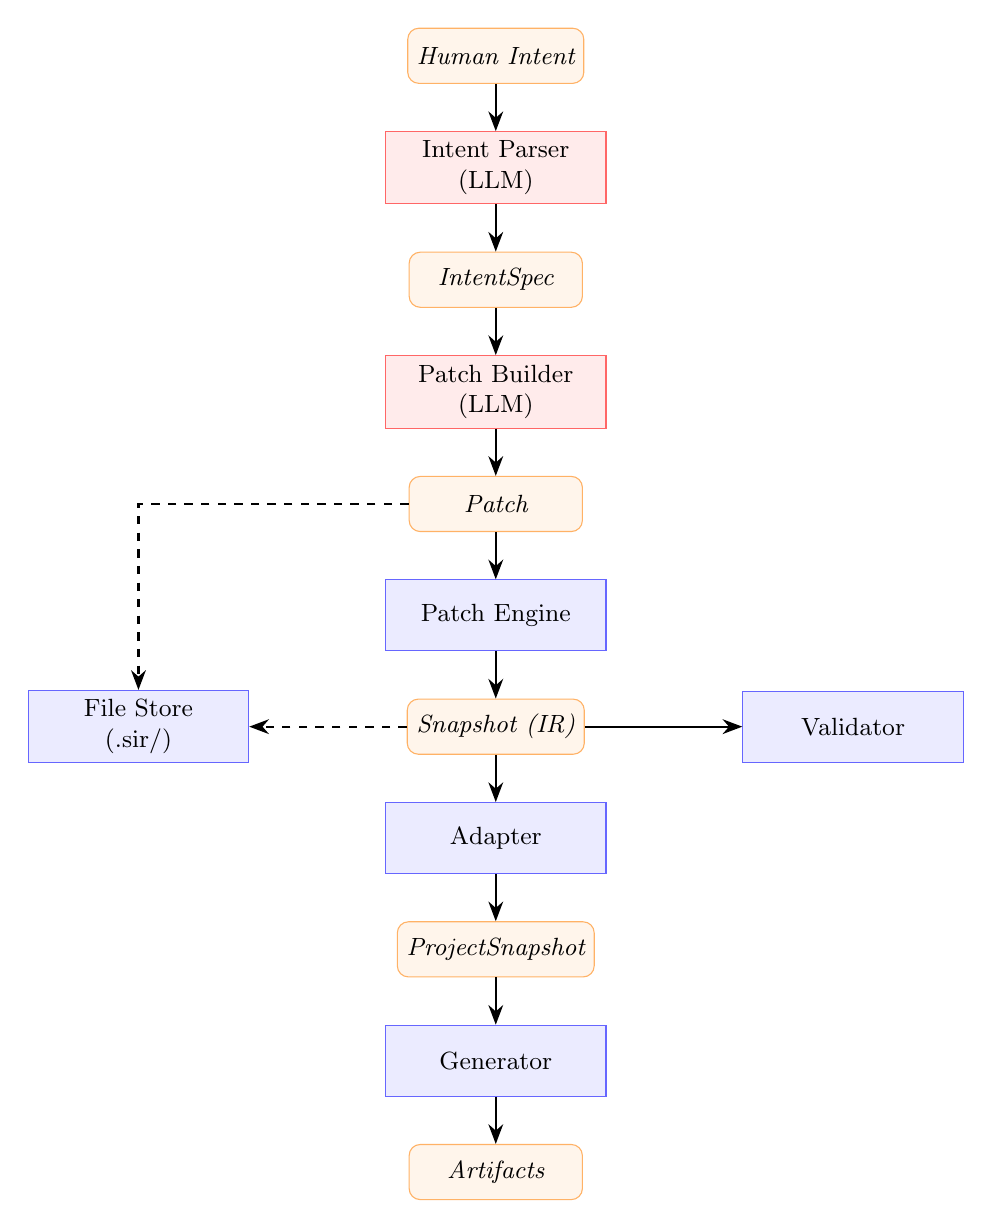
\begin{tikzpicture}[
    node distance=0.6cm and 1.2cm,
    stage/.style={rectangle, draw=blue!60, fill=blue!8, minimum width=2.8cm, minimum height=0.9cm, align=center, font=\small},
    data/.style={rectangle, rounded corners, draw=orange!60, fill=orange!8, minimum width=2.2cm, minimum height=0.7cm, align=center, font=\small\itshape},
    llm/.style={rectangle, draw=red!60, fill=red!8, minimum width=2.8cm, minimum height=0.9cm, align=center, font=\small},
    arrow/.style={-{Stealth[length=2.5mm]}, thick},
]

% Data nodes
\node[data] (intent) {Human Intent};
\node[llm, below=of intent] (parser) {Intent Parser\\(LLM)};
\node[data, below=of parser] (spec) {IntentSpec};
\node[llm, below=of spec] (builder) {Patch Builder\\(LLM)};
\node[data, below=of builder] (patch) {Patch};
\node[stage, below=of patch] (engine) {Patch Engine};
\node[data, below=of engine] (snapshot) {Snapshot (IR)};

% Right column
\node[stage, right=2cm of snapshot] (validator) {Validator};
\node[stage, below=of snapshot] (adapter) {Adapter};
\node[data, below=of adapter] (projsnap) {ProjectSnapshot};
\node[stage, below=of projsnap] (generator) {Generator};
\node[data, below=of generator] (artifacts) {Artifacts};

% Store
\node[stage, left=2cm of snapshot] (store) {File Store\\(.sir/)};

% Arrows
\draw[arrow] (intent) -- (parser);
\draw[arrow] (parser) -- (spec);
\draw[arrow] (spec) -- (builder);
\draw[arrow] (builder) -- (patch);
\draw[arrow] (patch) -- (engine);
\draw[arrow] (engine) -- (snapshot);
\draw[arrow] (snapshot) -- (validator);
\draw[arrow] (snapshot) -- (adapter);
\draw[arrow] (adapter) -- (projsnap);
\draw[arrow] (projsnap) -- (generator);
\draw[arrow] (generator) -- (artifacts);
\draw[arrow, dashed] (snapshot) -- (store);
\draw[arrow, dashed] (patch) -| (store);

\end{tikzpicture}
\caption{SIR compilation pipeline. Red boxes indicate LLM-powered stages; blue boxes are deterministic stages; orange boxes are data artifacts. Dashed arrows indicate persistence.}
\label{fig:architecture}
\label{fig:pipeline}
\end{figure}

\subsection{Graph IR}

The core abstraction is a directed graph $G = (N, E)$ where:

\begin{itemize}
    \item $N$ is a set of typed nodes: $n = (id, kind, name, desc, props)$ where $kind \in \{$\texttt{system, module, component, interface, entity, capability, workflow, event, constraint}$\}$.
    \item $E$ is a set of typed directed edges: $e = (u, v, type)$ where $type \in \{$\texttt{contains, depends\_on, implements, emits, consumes, triggers, constrains}$\}$.
\end{itemize}

A \textbf{Snapshot} $S_v = (v, N, E, M)$ captures the graph at version $v$ with optional metadata $M$. The \texttt{contains} edges form a tree (DAG constraint enforced by the validator) representing the compositional hierarchy: System $\supset$ Module $\supset$ Component/Entity/Interface/Workflow.

\textbf{Design rationale.} We chose a graph IR over an AST-based representation because software architecture is fundamentally a graph problem---modules depend on each other, components implement interfaces, workflows cross module boundaries. A tree-based IR would require awkward cross-references, while the graph naturally captures these relationships.

\subsection{Patch Semantics}

A Patch $P = (desc, [op_1, \ldots, op_k])$ is an ordered sequence of atomic operations:

\begin{itemize}
    \item \texttt{add\_node}$(n)$: Add node $n$ to $N$. Fails if $n.id \in \{m.id : m \in N\}$.
    \item \texttt{remove\_node}$(id)$: Remove node with given $id$ from $N$, and cascade-remove all edges referencing $id$.
    \item \texttt{update\_node}$(id, fields)$: Partial update of node fields.
    \item \texttt{add\_edge}$(u, v, type)$: Add edge. Fails if $u \notin N$ or $v \notin N$.
    \item \texttt{remove\_edge}$(u, v)$: Remove edge matching source and target.
\end{itemize}

The patch application function is deterministic:
$$\texttt{apply}: (S_v, P) \rightarrow S_{v+1}$$

Operations are applied sequentially, allowing later operations to reference nodes added by earlier ones in the same patch. This ordering constraint is communicated to the LLM via the prompt.

\subsection{Validation}

The validator enforces structural invariants on any snapshot:

\begin{enumerate}
    \item \textbf{Uniqueness}: Exactly one \texttt{system} node; all node IDs unique.
    \item \textbf{Referential integrity}: No dangling edges (all edge endpoints exist in $N$).
    \item \textbf{Acyclicity}: The \texttt{contains} subgraph must be a DAG.
    \item \textbf{Connectivity}: Orphan nodes (no edges) trigger warnings.
\end{enumerate}

Validation runs after every patch application, before persistence. This provides a ``type checker'' for the architectural IR---invalid transformations are rejected before code generation.

\subsection{Adapter Lowering}

The adapter stage performs \emph{lowering}---transforming the abstract IR into a project-specific representation with concrete file paths. The \texttt{GenericAdapter} implements a convention-based mapping:

\begin{equation}
\texttt{lower}: S \rightarrow PS = \{(n.id, n.kind, n.name, \texttt{path}(n)) : n \in N \setminus \{system\}\}
\end{equation}

where $\texttt{path}(n)$ is computed by walking the \texttt{contains} edge hierarchy to find the parent module and applying naming conventions (Table~\ref{tab:paths}).

\begin{table}[h]
\centering
\caption{Path generation rules in the Generic Adapter.}
\label{tab:paths}
\begin{tabular}{@{}ll@{}}
\toprule
\textbf{NodeKind} & \textbf{Path Pattern} \\
\midrule
Module & \texttt{\{snake\_name\}/} \\
Component & \texttt{\{module\}/components/\{name\}.py} \\
Entity & \texttt{\{module\}/models.py} \\
Interface & \texttt{\{module\}/services/\{name\}.py} \\
Workflow & \texttt{\{module\}/workflows/\{name\}.py} \\
\bottomrule
\end{tabular}
\end{table}

This separation allows different adapters for different project styles (e.g., a Django adapter, a microservices adapter) without changing the IR or the LLM prompts.

\subsection{Code Generation}

The generator emits source files from the \texttt{ProjectSnapshot}. The current \texttt{PythonGenerator} produces structural skeletons:

\begin{itemize}
    \item \textbf{Entity} $\rightarrow$ Python \texttt{@dataclass} with typed fields
    \item \textbf{Component} $\rightarrow$ Class with method stubs
    \item \textbf{Interface} $\rightarrow$ Abstract base class (\texttt{ABC}) with \texttt{@abstractmethod}
    \item \textbf{Workflow} $\rightarrow$ Function with step annotations
\end{itemize}

Multiple entities within the same module are merged into a single \texttt{models.py} file. The generator also creates Python package structure (\texttt{\_\_init\_\_.py} files).

\section{Implementation}

SIR is implemented in Python 3.12 using:
\begin{itemize}
    \item \textbf{Pydantic v2} for all data models with JSON serialization
    \item \textbf{NetworkX} for graph operations and DAG validation
    \item \textbf{Click} for the CLI interface
    \item \textbf{Anthropic SDK} for Claude API integration
\end{itemize}

The codebase comprises approximately 800 lines of core logic and 600 lines of tests, organized into 8 modules. The test suite contains 78 test cases covering all non-LLM components, achieving full path coverage for the deterministic pipeline stages.

\subsection{Persistence Model}

State is persisted in a \texttt{.sir/} directory (analogous to \texttt{.git/}):

\begin{lstlisting}[language=bash]
.sir/
  config.json           # Project metadata
  snapshots/
    v1.json             # Version history
    v2.json
    current.json        # Latest snapshot
  patches/
    patch_0000.json     # Applied patches
    patch_0001.json
\end{lstlisting}

This enables snapshot versioning, patch history review, and potential rollback---features that direct code generation cannot provide.

\section{Evaluation}

\subsection{Pipeline Correctness}

We validate the pipeline through comprehensive testing:

\begin{table}[h]
\centering
\caption{Test coverage summary.}
\label{tab:tests}
\begin{tabular}{@{}lcc@{}}
\toprule
\textbf{Module} & \textbf{Tests} & \textbf{Pass Rate} \\
\midrule
IR Schema & 8 & 100\% \\
IR Graph & 8 & 100\% \\
IR Validator & 7 & 100\% \\
Patch Engine & 11 & 100\% \\
File Store & 7 & 100\% \\
Adapter & 12 & 100\% \\
Generator & 10 & 100\% \\
CLI & 8 & 100\% \\
End-to-End & 5 & 100\% \\
\midrule
\textbf{Total} & \textbf{78} & \textbf{100\%} \\
\bottomrule
\end{tabular}
\end{table}

\subsection{End-to-End Demonstration}

We demonstrate the pipeline with a hand-crafted patch (simulating LLM output) that creates an authentication module with 6 nodes and 9 edges. The pipeline:

\begin{enumerate}
    \item Applies the patch to an initial snapshot (1 node $\rightarrow$ 7 nodes)
    \item Validates the resulting graph (no errors, no warnings)
    \item Lowers through the generic adapter (6 project nodes with paths)
    \item Generates 5 Python files with correct structure:
    \begin{itemize}
        \item \texttt{auth/models.py} --- \texttt{User} and \texttt{Session} dataclasses
        \item \texttt{auth/components/login.py} --- \texttt{Login} class with methods
        \item \texttt{auth/services/auth\_service.py} --- \texttt{AuthService} ABC
        \item \texttt{auth/workflows/login\_flow.py} --- \texttt{login\_flow()} function
    \end{itemize}
\end{enumerate}

Incremental patches (adding a component to an existing module) correctly update the snapshot without affecting existing nodes, demonstrating the composability of the patch model.

\section{Discussion}

\subsection{Advantages of the Compiler Metaphor}

\textbf{Separation of concerns.} The LLM handles \emph{what} (intent $\rightarrow$ architecture) while deterministic code handles \emph{how} (architecture $\rightarrow$ files). This mirrors the frontend/backend split in traditional compilers.

\textbf{Validation as type checking.} The validator acts as a type checker for the IR, catching structural errors before code generation. An LLM might hallucinate a reference to a non-existent node; the validator catches this deterministically.

\textbf{Incrementality.} Patches are additive. Instead of regenerating the entire codebase, we apply targeted modifications to the graph and regenerate only affected files.

\textbf{Traceability.} Every artifact can be traced back through: file $\leftarrow$ ProjectNode $\leftarrow$ IR Node $\leftarrow$ Patch $\leftarrow$ IntentSpec $\leftarrow$ human request.

\textbf{Testability.} By confining LLM non-determinism to two stages (intent parsing, patch building), the remaining 6 stages are fully deterministic and testable.

\subsection{Limitations and Future Work}

\textbf{Code body generation.} The current MVP generates structural skeletons only. A natural extension is a ``code filling'' pass where an LLM generates method implementations given the skeleton and architectural context.

\textbf{Multi-language support.} The adapter/generator separation makes this architecturally straightforward---a \texttt{TypeScriptGenerator} or \texttt{GoGenerator} would operate on the same \texttt{ProjectSnapshot}.

\textbf{Optimization passes.} The compiler analogy suggests architectural optimization: detecting redundant dependencies, merging similar components, splitting oversized modules. These could be implemented as graph rewriting rules.

\textbf{Bidirectional synchronization.} Currently, SIR generates code from the IR graph. A reverse direction---parsing existing code to reconstruct the IR---would enable SIR to work with existing codebases.

\textbf{Formal verification.} The graph IR is amenable to formal property checking (e.g., ``every interface has at least one implementation'', ``no module depends on a module that depends on it'').

\section{Related Work}

\textbf{LLM code generation.} Systems like Copilot~\citep{chen2021evaluating}, CodeGen~\citep{nijkamp2023codegen}, and AlphaCode~\citep{li2022alphacode} perform direct code generation. SIR complements these by providing an architectural layer above raw code generation.

\textbf{Program synthesis.} Classical program synthesis~\citep{gulwani2017program} uses formal specifications. SIR's IntentSpec serves a similar role but accepts natural language, leveraging LLMs as the ``synthesis engine.''

\textbf{Model-driven engineering.} MDE tools like EMF~\citep{steinberg2008emf} use metamodels to generate code. SIR's IR is conceptually similar to a metamodel, but uses LLMs instead of manual modeling.

\textbf{Software architecture recovery.} Tools that extract architectural models from code~\citep{garcia2013comparative} solve the inverse problem. Combining them with SIR would enable bidirectional synchronization.

\textbf{LLM agents.} Agent frameworks like AutoGPT, MetaGPT~\citep{hong2023metagpt}, and ChatDev~\citep{qian2024chatdev} orchestrate LLMs for software tasks. SIR differs by introducing a formal IR and compiler-style pipeline rather than free-form agent interaction.

\section{Conclusion}

Software Intent Runtime demonstrates that the compiler metaphor provides a powerful organizing principle for LLM-driven software engineering. By introducing a graph-based intermediate representation, a patch-based mutation model, and a multi-stage pipeline with clear separation of concerns, SIR achieves properties that direct code generation cannot: structural validation, incremental modification, full traceability, and deterministic testability of non-LLM stages. We believe this architecture points toward a future where LLMs serve not as code generators, but as \emph{software compilers}---translating human intent through principled intermediate representations into reliable software artifacts.

\bibliographystyle{plainnat}
\begin{thebibliography}{10}

\bibitem[Chen et al., 2021]{chen2021evaluating}
Chen, M., Tworek, J., Jun, H., et al. (2021).
\newblock Evaluating large language models trained on code.
\newblock \emph{arXiv preprint arXiv:2107.03374}.

\bibitem[Nijkamp et al., 2023]{nijkamp2023codegen}
Nijkamp, E., Pang, B., Hayashi, H., et al. (2023).
\newblock CodeGen: An open large language model for code with multi-turn program synthesis.
\newblock \emph{ICLR 2023}.

\bibitem[Li et al., 2022]{li2022alphacode}
Li, Y., Choi, D., Chung, J., et al. (2022).
\newblock Competition-level code generation with AlphaCode.
\newblock \emph{Science}, 378(6624):1092--1097.

\bibitem[Gulwani et al., 2017]{gulwani2017program}
Gulwani, S., Polozov, O., and Singh, R. (2017).
\newblock Program synthesis.
\newblock \emph{Foundations and Trends in Programming Languages}, 4(1-2):1--119.

\bibitem[Steinberg et al., 2008]{steinberg2008emf}
Steinberg, D., Budinsky, F., Paternostro, M., and Merks, E. (2008).
\newblock \emph{EMF: Eclipse Modeling Framework}.
\newblock Addison-Wesley Professional.

\bibitem[Garcia et al., 2013]{garcia2013comparative}
Garcia, J., Ivkovic, I., and Medvidovic, N. (2013).
\newblock A comparative analysis of software architecture recovery techniques.
\newblock \emph{ASE 2013}, pages 486--496.

\bibitem[Hong et al., 2023]{hong2023metagpt}
Hong, S., Zhuge, M., Chen, J., et al. (2023).
\newblock MetaGPT: Meta programming for a multi-agent collaborative framework.
\newblock \emph{arXiv preprint arXiv:2308.00352}.

\bibitem[Qian et al., 2024]{qian2024chatdev}
Qian, C., Liu, W., Liu, H., et al. (2024).
\newblock ChatDev: Communicative agents for software development.
\newblock \emph{ACL 2024}.

\end{thebibliography}

\appendix

\section{IR Node and Edge Type Definitions}

\begin{table}[h]
\centering
\caption{Complete NodeKind enumeration.}
\begin{tabular}{@{}lp{8cm}@{}}
\toprule
\textbf{Kind} & \textbf{Description} \\
\midrule
\texttt{system} & Root node representing the entire software system \\
\texttt{module} & A cohesive unit of functionality (e.g., ``authentication'') \\
\texttt{component} & An executable unit within a module (e.g., ``login handler'') \\
\texttt{interface} & A contract defining a service boundary \\
\texttt{entity} & A data model or domain object \\
\texttt{capability} & A discrete ability the system provides \\
\texttt{workflow} & A multi-step process or business flow \\
\texttt{event} & A signal emitted or consumed by components \\
\texttt{constraint} & A rule or invariant that must be maintained \\
\bottomrule
\end{tabular}
\end{table}

\begin{table}[h]
\centering
\caption{Complete EdgeType enumeration.}
\begin{tabular}{@{}lp{8cm}@{}}
\toprule
\textbf{Type} & \textbf{Description} \\
\midrule
\texttt{contains} & Compositional hierarchy (must form a DAG) \\
\texttt{depends\_on} & Runtime or compile-time dependency \\
\texttt{implements} & A component realizes an interface \\
\texttt{emits} & A component produces an event \\
\texttt{consumes} & A component reacts to an event \\
\texttt{triggers} & One workflow/component initiates another \\
\texttt{constrains} & A constraint applies to a node \\
\bottomrule
\end{tabular}
\end{table}

\end{document}
